\documentclass[12pt]{article}
\usepackage{amssymb,amsmath,latexsym, braket,caption, subcaption}
\usepackage{tikz, pgfplots, graphicx, standalone}
\newcommand{\dt}[1]{\frac{\mathrm d #1}{\mathrm dt}}
%\usetikzlibrary{external}
%\tikzexternalize[prefix=i/]
\begin{document}

\title{The Kuramoto Model}
\author{Manish Goregaokar}

\maketitle

\begin{abstract}
Synchronization is a common phenomenon occurring with coupled oscillators, where over time their phases become locked. It is observed in a wide range of situations, from the tidal locking of the moon to fireflies to neural clusters. This report gives an overview of this phenomenon, with specific focus on the Kuramoto model.
\end{abstract}
\tableofcontents
\section{Introduction}

In 1665, Christian Huygens made the first recorded observation and analysis of synchronization\cite{bennett2002huygens}. He noticed that a pair of pendulums kept in the same housing would gradually start moving in unison regardless of their initial conditions. Additionally, if perturbed after the synchronization, the pendulums would re-synchronize. He attributed this effect to the motion of the beam connecting the two, but did not manage to make a complete model of this phenomenon.

The field was quite dormant until the early 1900s, when J. Vincent\cite{vincent1919some}, Van Der Pol\cite{van1920theory}, and E. Appleton\cite{appleton1922automatic} experimented with electrical circuits involving triode oscillators.

After this, there has been a myriad of topics in which synchronization has been studied, including in many electrical, chemical, and biological systems. Additionally, the phenomenon has many applications --- for example, pacemakers are a driving oscillator to the heart in a synchronized system.

\section{Basics}
\subsection{Coupled oscillators}
Systems which individually behave as oscillators can be "coupled", such that at least one of them is exposed to an effect dependent on the phases of the two oscillators. Usually this effect is monotonic and dependent on the phase difference only. Coupling can be one way or two way ("mutual coupling"). In the one-way case we have a "driving oscillator" which is unaffected by the other oscillator(s), and the other oscillator(s) are known as the "driven oscillator(s)".

For example, for a pair of oscillators, unidirectional coupling could have the equations:
\begin{align*}
\dt{\phi_1} &= \omega \\
\dt{\phi_2} &= \omega - k\sin(\phi_2 - \phi_1)
\end{align*}

whereas bidirectional coupling would be:
\begin{align*}
\dt{\phi_1} &= \omega + k\sin(\phi_2 - \phi_1)\\
\dt{\phi_2} &= \omega - k\sin(\phi_2 - \phi_1)
\end{align*}

In cases where one oscillator has no external effects, sometimes it is considered as ``external forcing".


Oscillators need not have the same $\omega$ (or in general, the same state-space portraits) to be coupled.

\subsection{Synchronization}
Synchronization is simply the process by which a number of coupled oscillators begin to move in lockstep (either in phase or anti-phase) after being allowed to oscillate for some period of time.

For synchronization to happen, the system must be made of coupled oscillators; i.e. the components, when uncoupled, should individually be autonomous oscillators.

A very simple example of synchronization would be where there is a pair of oscillators coupled unidirectionally. It is usually convenient to abstract the driving oscillator away as a "driving force". This makes the system non-autonomous but easier to understand. When the driving force has the same frequency as the oscillator, it is usually guaranteed that there will be phase locking; i.e. the oscillators will eventually have a $0$ or $\pi$ phase difference.

\begin{figure}
\centering
\begin{subfigure}[b]{0.4\textwidth}
\includestandalone[mode=image,width=\textwidth]{i/detuning}
\caption{perfect and imperfect synchronization}\label{fig:detuning}
\end{subfigure}
\begin{subfigure}[b]{0.4\textwidth}
\includestandalone[mode=image,width=\textwidth]{i/arnold}
\caption{Arnold tongue}\label{fig:arnold}
\end{subfigure}
\end{figure}

When the driving force has a different frequency, we have more robust behavior. For low values of the frequency difference, we get \emph{frequency locking} (usually coupled with phase locking) where the driven oscillator eventually oscillates at the driving frequency. However, at higher frequency differences, we no longer have perfect synchronization, however the driven frequency is brought closer to the final one. We can see this behavior in Figure \ref{fig:detuning}, where there is perfect synchronization in a region around $\omega_{\rm driving}$,outside of which the amount of synchronization gradually drops off. The width of this region increases with an increasing driving amplitude. If we plot the region synchronization with amplitude, we get something like Figure \ref{fig:arnold}, known as an \emph{Arnold tongue}\cite{pikovsky2001synchronization}.

Even if the two frequencies are not close, we can still have some synchronization if their harmonics are close. The two frequencies will then attempt to synchronize in a way so that those two harmonics come closer or become equal.


\subsection{Ensemble of oscillators}
\begin{figure}
\centering
\includestandalone[mode=image]{i/almostfull}
\caption{Almost full synchronization}\label{fig:fullgraph}
\end{figure}

\begin{figure}
\centering
\includestandalone[mode=image]{i/partial}

\caption{Partial synchronization}\label{fig:partialgraph}
\end{figure}

\begin{figure}
\centering
\includestandalone[mode=image]{i/nonesync}

\caption{No synchronization}\label{fig:nograph}
\end{figure}
Typically, most synchronizing real systems can be modeled with an \emph{ensemble} of coupled oscillators. Coupling may or may not be global.

In such an ensemble, synchronization can be "partial"; i.e. there are some elements of synchronization to be found, but it is still not fully synchronized. For example, in Figure \ref{fig:fullgraph}, we have the time series for a system of almost completely synchronized oscillators (Complete full synchronization would be where the time series for all oscillators are equal or opposite).

Contrast this with Figure \ref{fig:nograph}, where there is no synchronization at all. While there are times in which the oscillators seem to come close to synchronization, these do not last. However, in Figure \ref{fig:partialgraph}, we have what is known as ``partial synchronization". The majority of the oscillators here are close to the ``mean" time
 series, though there may be a minority of oscillators which are out of phase. It is not necessary that the \emph{sames} oscillators will continue to stay somewhat in phase; usually the number of partially synchronized oscillators is approximately constant, however individual oscillators alternate between being in phase and out of phase with the rest.



\section{The Kuramoto Model}
The Kuramoto model was first proposed in 1975 by Yoshiki Kuramoto\cite{kuramoto1975proceedings}
The Kuramoto model models an ensemble of coupled oscillators
$$\dot{\theta_i} = \omega_i + \frac{K}{N}\sum_j a_{ij}\sin(\theta_j - \theta_i) $$

Here, $N$ is the number of oscillators, $K$ is the coupling parameter, and $a_{ij}$ determines how the network of oscillators is coupled. Usually, $a_{ij}=a_{ji}$, and its value is either 0 or 1, denoting uncoupled and coupled oscillators respectively. This matrix defines the topology of the system. Interesting behavior can be observed when the $\omega_i$s are different.

\subsection{Order parameter}
An important way to measure the ``amount" of synchronization. is via something known as the \emph{order parameter}. For an ensemble of oscillators with phases $\theta_i$, the Kuramoto order parameter is 

$$r = \frac1{N}\left|\sum_i e^{i\theta_i}\right|$$

For a completely synchronized system, this parameter is 1, and for an unsynchronized system it will usually be a low value. Partial synchronization is when the value is not small on an average.
\subsection{Analysis of a globally coupled Kuramoto system}


I simulated a globally coupled Kuramoto system of 30 oscillators, with a 10\% variation in the $\omega_i$s, and varied $K$. For very low $K$, we get no synchronization as seen in Figure \ref{fig:plot:nosynchro}. While the order parameter may rise to larger values (sometimes even coming close to 1), \emph{on an average} the order parameter stays very low.

While in some cases for partial synchronization the order parameter settles on a particular value and doesn't vary (Figure \ref{fig:plot:partial2}), this is not true in the general case. For example, for lower values of $K$ we can get a time evolution like in Figure \ref{fig:plot:partial1}, where the order parameter doesn't settle, but on an average is an appreciable value. For higher $K$ values, we can have a time evolution similar to that in Figure \ref{fig:plot:partial1}, where the order parameter does settle to a single, large value.
\begin{figure}
\centering
\begin{subfigure}[b]{0.4\textwidth}
\centering
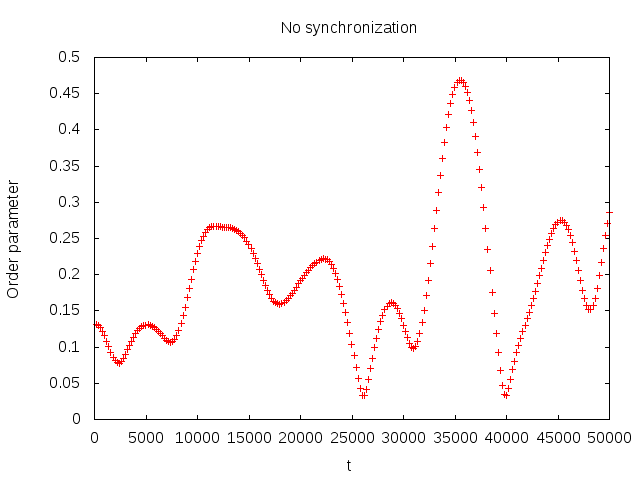
\includegraphics[width=\textwidth]{data/strange}
\caption{No synchronization with $K=0.01$}
\label{fig:plot:nosynchro}
\end{subfigure}
\begin{subfigure}[b]{0.4\textwidth}
\centering
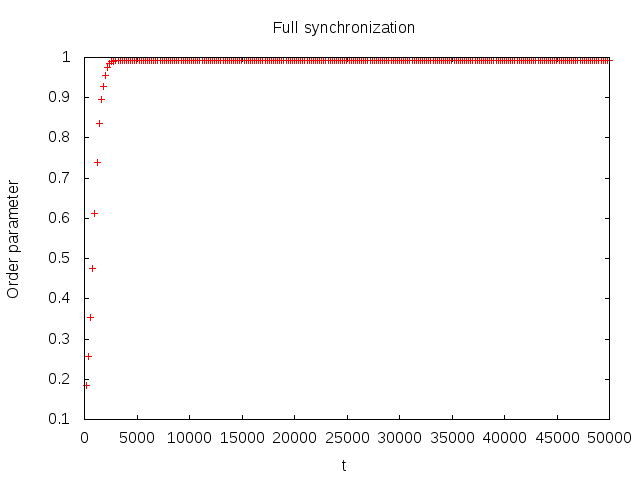
\includegraphics[width=\textwidth]{data/full}
\caption{Full synchronization with $K=0.2$}
\label{fig:plot:full}
\end{subfigure}
\begin{subfigure}[b]{0.4\textwidth}
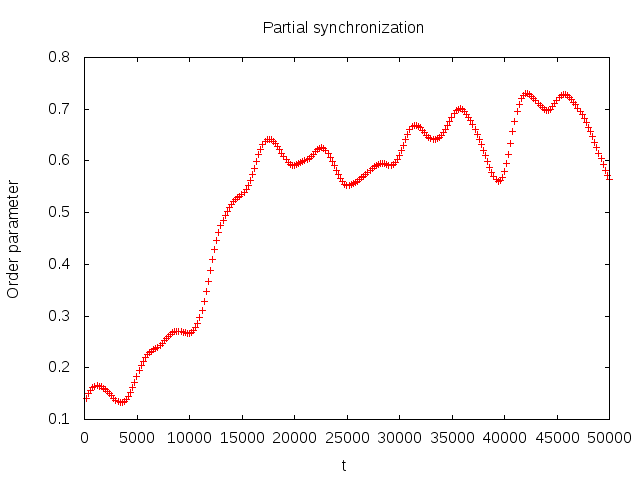
\includegraphics[width=\textwidth]{data/partialsm}
\caption{Partial synchronization with $K=0.05$}
\label{fig:plot:partial1}
\end{subfigure}
\begin{subfigure}[b]{0.4\textwidth}
\centering
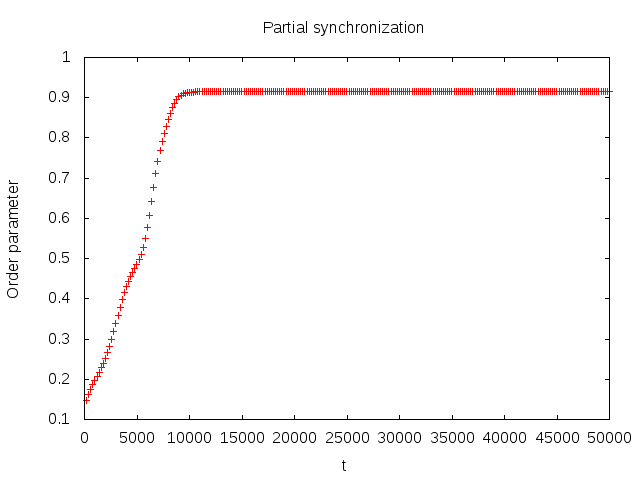
\includegraphics[width=\textwidth]{data/partialmore}
\caption{Partial synchronization with $K=0.07$}
\label{fig:plot:partial2}
\end{subfigure}
\caption{Time series for various levels of coupling}
\end{figure}

Finally, we can have full synchronization with very large values of the order parameter, as seen in Figure \ref{fig:plot:full}. The ensemble quickly reaches an order parameter of $1$ and stays there.

If we plot the variation of the order parameter with the coupling constant, we get a graph like the one in Figure \ref{fig:plot:ovc}. Note that we have to take a time average of the order parameter (without transients) to get most of the points in this graph since the order parameter for these points is not constant but rather oscillates erratically around some value. Generally, the lower the coupling constant, the more the variation in the order parameter.

\begin{figure}
\centering
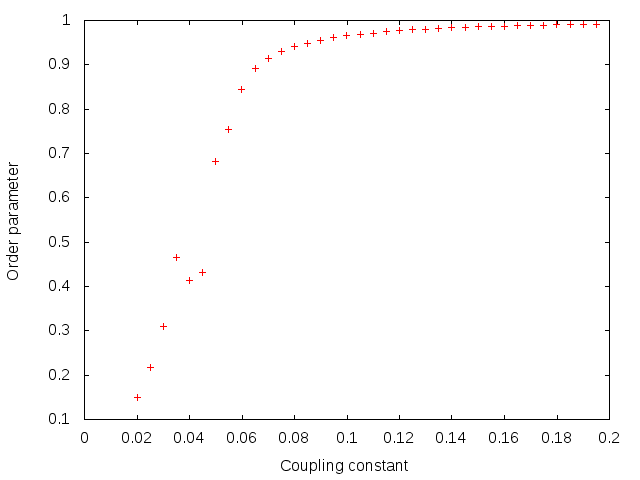
\includegraphics[scale=0.5]{data/ovcoupling}
\caption{Variation of order parameter with coupling constant}
\label{fig:plot:ovc}
\end{figure}
\bibliographystyle{abbrv}
\bibliography{bib}

\subsection{Mathematical analysis}

Usually, we are interested in the systems where the
\end{document}